
% Chapter 1

\chapter{Introducción general} % Main chapter title
En el presente capítulo se presenta una descripción del contexto y la importancia de contar con información precisa sobre el consumo energético. Además, se aborda la motivación detrás del trabajo, subrayando la necesidad de reducir el impacto ambiental y los costos asociados al consumo eléctrico, se presentan los objetivos y el alcance y se detallan las metas específicas. Finalmente, se realiza una análisis sobre el estado del arte de las tecnologías relacionadas existentes en la actualidad.

\label{Chapter1} % For referencing the chapter elsewhere, use \ref{Chapter1} 
\label{IntroGeneral}


%----------------------------------------------------------------------------------------

% Define some commands to keep the formatting separated from the content 
\newcommand{\keyword}[1]{\textbf{#1}}
\newcommand{\tabhead}[1]{\textbf{#1}}
\newcommand{\code}[1]{\texttt{#1}}
\newcommand{\file}[1]{\texttt{\bfseries#1}}
\newcommand{\option}[1]{\texttt{\itshape#1}}
\newcommand{\grados}{$^{\circ}$}

%----------------------------------------------------------------------------------------

%\section{Introducción}

%----------------------------------------------------------------------------------------

\section{Sistema de monitoreo de consumo eléctrico}
Tener información es crucial para la toma de decisiones ya que mejora la calidad de las mismas al basarlas en hechos y datos concretos. Permite identificar oportunidades y riesgos, reduce incertidumbres, facilita la planificación estratégica y el uso eficiente de los recursos. 

En el ámbito de la energía, y dado el contexto actual, contar con datos de buena calidad se ha vuelto particularmente importante. En las últimas décadas, la creciente demanda de energía eléctrica ha generado preocupaciones significativas a nivel mundial. Este incremento en el consumo energético, impulsado por el crecimiento poblacional, la industrialización y la expansión de tecnologías dependientes de la electricidad, ha llevado a una mayor explotación de recursos naturales y un aumento de las emisiones de gases de efecto invernadero, como se observa en la figura \ref{fig:emisionesco2}. Estos factores han contribuido al cambio climático, provocando impactos ambientales que van desde el calentamiento global hasta la pérdida de biodiversidad y eventos climáticos extremos.

\newpage

\begin{figure}[ht]
	\centering
	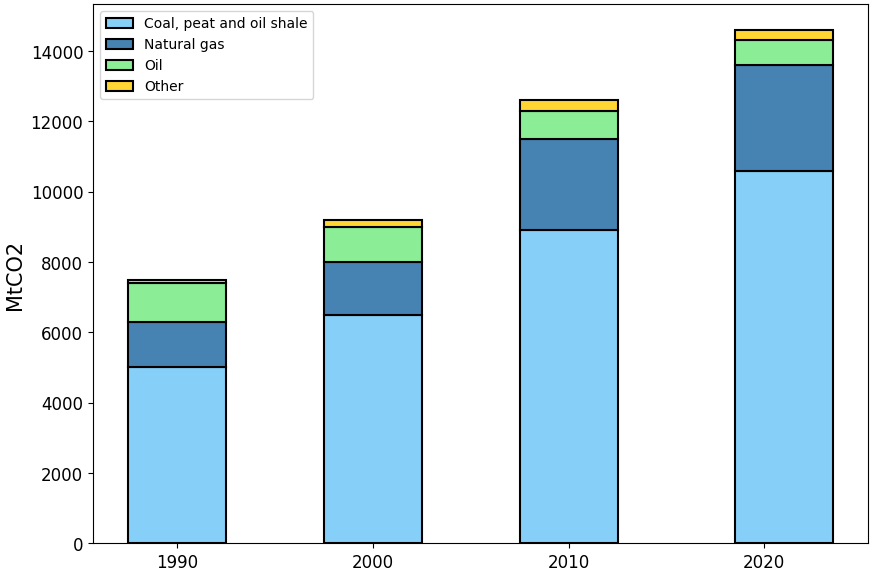
\includegraphics[width=1\textwidth]{./Figures/co2_emissions.png}
	\caption[Emisiones de $CO_2$ por la generación de electricidad.]{Emisiones de $CO_2$ por la generación de electricidad y calor por fuente de energía a nivel global\footnotemark.}
	\label{fig:emisionesco2}
	
\end{figure}

\footnotetext{IEA (2023), Greenhouse Gas Emissions from Energy Data Explorer, IEA, Paris \url{https://www.iea.org/data-and-statistics/data-tools/greenhouse-gas-emissions-from-energy-data-explorer}}

Según un informe de la \textit{International Energy Agency} (IEA) \cite{ieareport}, y como se observa en la figura \ref{fig:demandaElectricidad}, se espera que el crecimiento de la demanda global de electricidad aumente del 2,6 \% en 2023 a un promedio del 3,2 \% en 2024-2025. El estudio también destaca que para 2025, la demanda aumentará en 2500 TWh con respecto a los niveles de 2022, lo que significa que en los próximos tres años, el aumento anual del consumo de electricidad será aproximadamente equivalente a la suma del consumo de Reino Unido y Alemania juntos.

\newpage

\begin{figure}[ht]
	\centering
	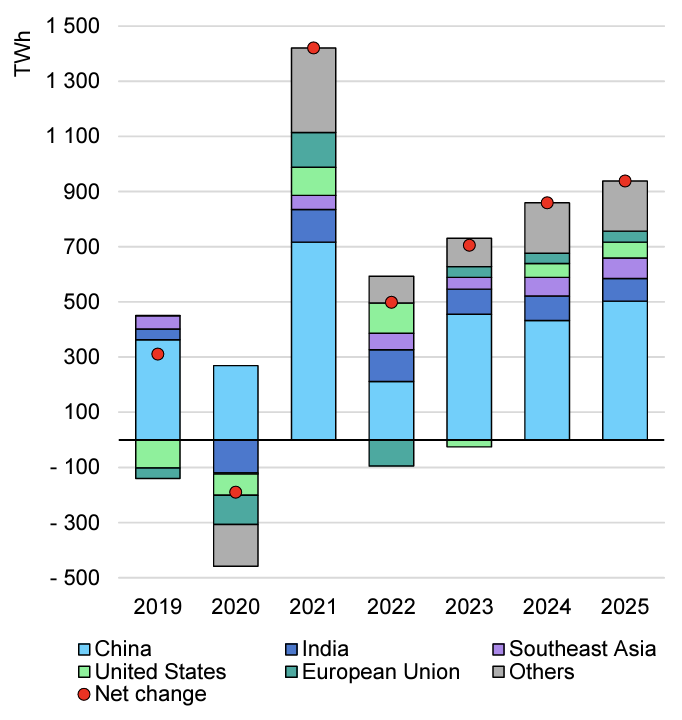
\includegraphics[width=.7\textwidth]{./Figures/year-on-year-change-in-electricity-demand-by-region-2019-2025.png}
	\caption[Cambio anual en la demanda de electricidad por región para el período 2019-2025.]{Cambio anual en la demanda de electricidad por región para el período 2019-2025\footnotemark.}
	\label{fig:demandaElectricidad}
\end{figure}

\footnotetext{IEA (2023), Year-on-year change in electricity demand by region, 2019-2025, IEA, Paris \url{https://www.iea.org/data-and-statistics/charts/year-on-year-change-in-electricity-demand-by-region-2019-2025}, Licence: CC BY 4.0}

Al mismo tiempo, el costo de la electricidad también ha experimentado un incremento significativo en los últimos años, impulsado por diversos factores como la creciente demanda, el aumento de precios de los combustibles utilizados para su generación y factores geopolíticos. Este aumento impacta directamente en el presupuesto de los hogares y en la competitividad de las industrias y la economía en general.

En este contexto, la eficiencia energética se ha convertido en una prioridad global. Gobiernos, organizaciones y consumidores buscan métodos para optimizar el uso de la energía y reducir su huella de carbono. 

Uno de los sectores donde esta optimización es crucial es el consumo eléctrico domiciliario. Los hogares representan una parte significativa del consumo energético total y, a menudo, carecen de herramientas eficaces para monitorear y gestionar su uso de electricidad. Esta falta de visibilidad y control sobre el consumo diario impide a los usuarios adoptar hábitos más sostenibles y económicos.

Para lograr una mayor eficiencia es vital poder contar con información en tiempo real relacionada al consumo de energía eléctrica. Tener estos datos permitiría, por ejemplo, identificar cuáles son los electrodomésticos y hábitos que más energía consumen o tomar decisiones informadas al reemplazar o adquirir nuevos dispositivos. Disponer de información adecuada puede ayudar a los hogares a enfocar los esfuerzos de ahorro energético, disminuir sus costos asociados y contribuir a la sostenibilidad ambiental.

\newpage
\section{Motivación}
La motivación del trabajo surge de la necesidad de abordar los desafíos previamente planteados relacionados con el consumo energético, la sostenibilidad ambiental y la economía doméstica. El sistema busca generar datos y proveer información para lograr una reducción de consumo eléctrico a partir de la adopción de prácticas más eficientes. Esta disminución y eficientización del consumo es clave ya que sirve para reducir el impacto ambiental relacionado con la generación y consumo de energía y para reducir costos.

\section{Objetivos y alcance}

\subsection{Objetivos}
El principal objetivo del trabajo es el diseño e implementación de un prototipo que permita, principalmente a usuarios domiciliarios, tener información sobre su consumo de electricidad para poder tomar decisiones inteligentes que apunten a reducir el uso de energía. El objetivo subyacente es asistir a los usuarios en la reducción de costos y generar un impacto positivo en el ambiente. Este objetivo macro se desglosa en varios objetivos específicos:

\begin{itemize}
	\item Medir variables eléctricas esenciales como tensión, corriente, potencia, frecuencia y factor de potencia.
	
	\item Asegurar que el dispositivo transmita los datos de manera confiable a un servidor en la nube para su procesamiento, almacenamiento y posterior consumo.

	\item  Proveer al usuario una interfaz intuitiva que le permita acceder a sus datos de consumo eléctrico de manera clara y comprensible.

	\item Ofrecer herramientas analíticas para identificar patrones de consumo y sugerir acciones para mejorar la eficiencia energética. 
	
	\item Fomentar el uso responsable de la energía mediante recomendaciones basadas en datos precisos.
	
	\item Educar a los usuarios sobre su consumo energético y las maneras de optimizarlo, para contribuir a la reducción de costos y del impacto ambiental.
	
	\item Asegurar que el sistema sea escalable para adaptarse a diferentes volúmenes de datos y a un número creciente de usuarios.
	
	\item Mantener la accesibilidad y facilidad de uso del sistema, para garantizar que usuarios sin conocimientos técnicos avanzados puedan beneficiarse de la herramienta.
\end{itemize}

\subsection{Alcance}

El alcance del trabajo abarca desde el diseño inicial hasta la implementación y despliegue de un sistema de monitoreo. Este sistema incluye varios componentes y fases clave de desarrollo:

\begin{itemize}
	\item Diseño y desarrollo del dispositivo de medición:
		\begin{itemize}
		\item Selección de componentes de hardware y sensores adecuados para la medición de variables eléctricas.
		\item Programación del dispositivo para la captura precisa de datos y su transmisión mediante conexión Wi-Fi.
		\end{itemize}
	\item Implementación de un servidor:
		\begin{itemize}
		\item Configuración de una base de datos relacional para el almacenamiento seguro y eficiente de grandes volúmenes de datos.
		\item Desarrollo de endpoints HTTP que permitan operaciones CRUD \cite{crud} sobre los datos y la gestión de usuarios.
		\item Implementación de un broker MQTT.
		\end{itemize}
	\item Desarrollo de la plataforma web:
	\begin{itemize}
		\item Creación de una interfaz de usuario intuitiva utilizando frameworks modernos.
		\item Integración de funcionalidades analíticas y visualización de datos, que faciliten la interpretación y el análisis del consumo eléctrico por parte de los usuarios.
	\end{itemize}
	\item Fase de pruebas y validación:
	\begin{itemize}
		\item Realización de pruebas unitarias y de integración para asegurar la correcta interacción entre el dispositivo de medición, el servidor en la nube y la plataforma web.
		\item Validación del sistema en un entorno real para garantizar su funcionalidad y eficacia.
	\end{itemize}
	\item Despliegue y mantenimiento:
	\begin{itemize}
		\item Implementación del sistema en un entorno operativo real, disponible para usuarios domésticos.
	\end{itemize}
\end{itemize} 


\newpage

\section{Estado del arte}

Existen diversas tecnologías y productos que permiten a los usuarios monitorizar y gestionar su uso de energía de manera eficiente. Estos dispositivos varían en capacidades, parámetros medidos, precios y características técnicas. 

A continuación, se presenta una comparativa de algunos de los productos más destacados en el mercado, evaluando sus capacidades, parámetros medidos, precios y especificaciones técnicas.

\begin{itemize}
    \item Sense Home Energy Monitor \cite{competencia1}: 
    Sense es una aplicación móvil que muestra cuánta energía están consumiendo el hogar y los dispositivos individuales en tiempo real. Ayuda a encontrar maneras de ahorrar dinero y reducir la huella de carbono, ofreciendo información personalizada y herramientas para rastrear los aparatos que más energía consumen.

    \item Emporia Vue \cite{competencia2}:
    el monitor de energía doméstica Emporia Vue permite monitorear el uso de energía en tiempo real e identificar cualquier consumo de energía innecesario, ayudando a ahorrar dinero. Es reconocido como el mejor monitor de energía doméstica del mercado y es líder en ventas en Amazon. Permite el monitoreo de hasta 16 circuitos individuales, con integración con asistentes de voz como Alexa para control y notificaciones.

    \item Aeotec Home Energy Meter \cite{competencia3}:
    los sensores pertenecientes a la familia Aeotec Home Energy Meter son compatibles con las tecnologías Zigbee o Z-Wave, y proporcionan datos vitales para hacer que una red doméstica sea verdaderamente inteligente. Los sensores no solo recopilan y transfieren datos, sino que también permiten activar automatizaciones vinculadas. Los datos recopilados también se utilizan para advertir, informar y proteger la instalación eléctrica en el caso que se den condiciones inusuales.

    \item TED Pro Home \cite{competencia4}:
    el T1500 es un medidor de potencia que mide con precisión el consumo de energía de los dispositivos. Tiene una funcionalidad que permite al usuario introducir el valor del kilowatt-hora (kWh) y, en base a esto, se estima el costo de la energía consumida por el electrodoméstico conectado. El T1500 también puede usarse para verificar la calidad de la energía al monitorear el tensión, la frecuencia y el factor de potencia entre otras variables. No posee forma de almacenamiento de datos históricos.

    \item Efergy Elite 4.0 \cite{competencia5}:
    este dispositivo permite ver cuánta electricidad se está usando en cualquier momento (costo y kW), ver datos promedio e históricos diarios, semanales o mensuales, configurar hasta 4 tarifas diferentes y múltiples monedas mundiales, y emitir alertas de audio frente a consumos de energía excesivos.
\end{itemize}

En la tabla \ref{tab:tablaComparativaProductos} se presenta en forma condensada la comparativa entre los distintos productos. Se consideran valores en dólares americanos (USD).

\begin{table}[h]
	\centering
        \caption[Productos actuales en el mercado]{Tabla comparativa de los productos similares presentes en el mercado.}
	\begin{tabular}{c c c c}    
		\toprule
		\textbf{Producto} 	 & \textbf{\makecell{Parámetros \\Medidos}} 		& \textbf{Precio} & \textbf{\makecell{Especificaciones \\Técnicas}}  \\
		\midrule
		\makecell{Sense Home \\Energy Monitor} & \makecell{V, A, W,\\ FP, Hz}   & \$ 300  & \makecell{Wi-Fi, detección de \\dispositivos, app móvil \\integrada, procesamiento edge.}\\	
  
		Emporia Vue	              & \makecell{V, A, W,\\ FP, Hz}   & \$ 100  & \makecell{Wi-Fi, 16 sensores de \\circuito, app móvil, \\integración con asistentes de voz.}\\
  
		\makecell{Aeotec Home \\Energy Meter}  & \makecell{V, A, W,\\ FP, Hz}   & \$ 130  & \makecell{Z-Wave, medición\\ de energía total y por fase.}\\

            TED 1500                  & \makecell{V, A, W,\\ FP, Hz}   & \$ 50   &\makecell{Pantalla LCD, batería\\ de respaldo, aviso \\de sobre tensión.}\\
            
            Efergy Elite 4.0          & \makecell{V, A, W,\\ FP, Hz}   & \$ 49   &\makecell{RF, pantalla LCD, \\almacenamiento de datos \\de hasta 24 meses.}\\
		\bottomrule
		\hline
	\end{tabular}
 	
	\label{tab:tablaComparativaProductos}
\end{table}

La selección de un sistema de monitoreo de consumo eléctrico depende de las necesidades específicas del usuario, incluyendo el nivel de detalle requerido, la facilidad de instalación y el presupuesto disponible. Los productos comparados ofrecen una gama de capacidades y características, desde la medición y visualización del consumo eléctrico en el propio dispositivo, hasta la detección avanzada de dispositivos, la integración con sistemas de domótica y la generación de informes. Esta comparativa proporciona una base para evaluar la solución presentada en el presente trabajo.

